\documentclass[a4paper,12pt]{report}

\usepackage{alltt, fancyvrb, url}
\usepackage{graphicx}
\usepackage{subfigure}
\usepackage{wrapfig}
\usepackage{algorithmic}
\usepackage[utf8]{inputenc}
\usepackage{fontenc}
\usepackage{amsmath,stmaryrd,mathtools,algorithm}
\usepackage{amssymb}
\usepackage{float}
\usepackage{hyperref}
\usepackage{listings}

% Remove option to use English naming
\usepackage[italian]{cleveref}

% Questo commentalo se vuoi scrivere in inglese.
\usepackage[italian]{babel}

\title{KeePassJ per\\``Programmazione ad Oggetti''}
 
\author{Di Santi Giovanni, Ercolani Francesco, Conti Massimiliano, Cellot Davide}
\date{\today}


\begin{document}
 
\maketitle

\tableofcontents

\chapter{Analisi}

\section{Requisiti}

Il gruppo si pone come obiettivo quello di realizzare un keepass per salvare
in modo sicuro le password. Al momento i keepass desktop più usati sono
\href{https://keepass.info/}{keepass2} e \href{https://keepassxc.org/}{keepassxc}.
TODO: scrivere descrizione più lunga.

\subsubsection{Requisiti funzionali}
\begin{itemize}
  \item Il database su cui sono salvate le password deve essere opportunamente
    autenticato e cifrato, in modo da non permettere a terze parti di leggere
    o manipolare il contenuto delle password.
  \item Gestione delle entry (add, edit, delete) con la possibilità di suddividere
    le entry in vari gruppi.
  \item Funzioni per generare in modo sicuro password e controllarne la validità.
  \item Possibilità di importare in chiaro un database in formato XML, in modo simile
    alla funzionalità di un keepass originale.
  \item Sezione Statistics che mostra le statistiche relative al proprio database (Es. il numero di account salvati)
\end{itemize}

\subsubsection{Requisiti non funzionali}
\begin{itemize}
  \item Possibilità di cifrare archivi esterni.
  \item Funzioni di sort e find per ordinare e cercare entry specifiche.
  \item Funzione expire che avvisa quando una password è da cambiare (es. 2 anni).
\end{itemize}

\section{Analisi e modello del dominio}

Nella creazione del database bisogna inserire una master password. Dopodiché è 
necessario configurare vari parametri, tra cui il cipher e la Key Derivation Function (KDF)
da usare. La KDF ha vari parametri opzionali da utilizzare per generare la key
in modo più sicuro (più rounds) o più veloce (più parallelismo).
Lo pseudocodice seguente spiega come la \textbf{KDF} e il \textbf{cipher} sono collegati:
\begin{lstlisting}
plaintext = "this is the plaintext"
key = KDF(password)
ciphertext = cipher.encrypt(key, plaintext)
assert plaintext == cipher.decrypt(key, ciphertext)
\end{lstlisting}
I vari parametri crittografici del database sono configurabili tramite \textbf{KDBHeader},
che vengono usati dalla classe \textbf{KDB} per effettuare l'encryption e la decryption
di array di byte arbitrari.
Per lavorare sul database in chiaro usiamo un ulteriore classe che è \textbf{DataBase}
che permettera di manipolare le entry e i gruppi.

\begin{figure}[h]
\centering{}
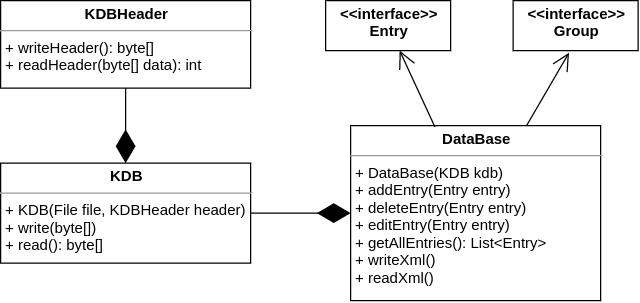
\includegraphics[width=\textwidth]{analysis}
\caption{rappresentazione UML dell'analisi del progetto}
\end{figure}

\chapter{Design}

\section{Architettura}

Per la realizzazione di KeePassJ abbiamo scelto di utilizzare il pattern architetturale
Model-View-Controller (MVC).

TODO: Inserire schema UML MVC.

\section{Design dettagliato}

TODO: Spiegare a grandi linee

\section*{Giovanni Di Santi}

Il mio compito principale del progetto è stato quello di gestire la parte crittografica e
definire la struttura dell'header del database.

\subsection*{CryptoCipher}

\textbf{CryptoCipher} è l'interfaccia che descrive i metodi necessari per effettuare
l'encryption e la decryption di un array di \texttt{byte}.\\
Ogni implementazione disponibile di questa interfaccia è un
\href{https://web.cs.ucdavis.edu/~rogaway/papers/ad.pdf}{AEAD Cipher} 
(Authenticated Encryption with Associated Data).\\
Ho scelto questo schema di encryption per rendere il database resistente ad 
attacchi del tipo \textbf{CCA} (Chosen Ciphertext Attack), cifrando il contenuto del
database e autenticando sia il contenuto che l'header (Associated Data).
\begin{figure}[h]
\centering{}
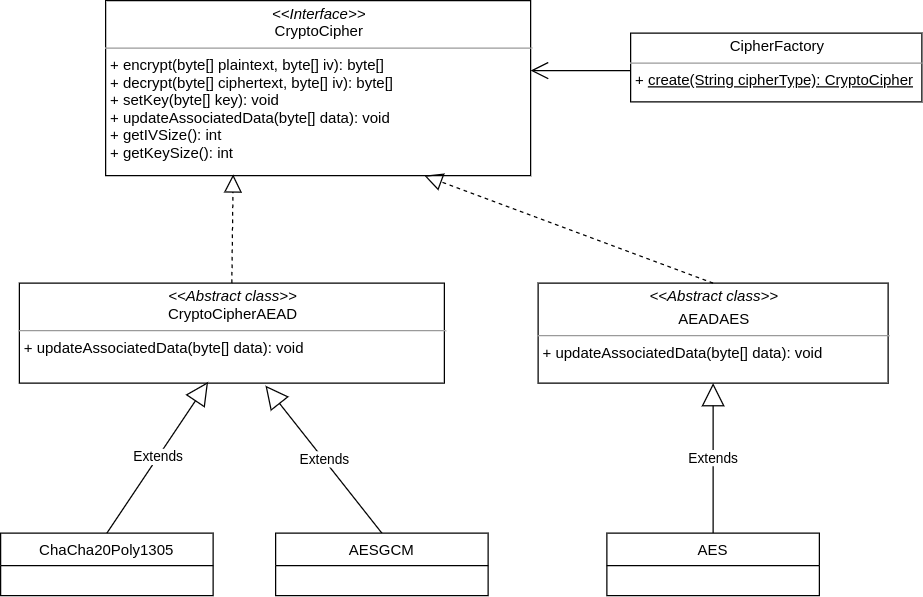
\includegraphics[width=\textwidth]{crypto-cipher}
\caption{rappresentazione UML del pattern factory per creare un CryptoCipher}
\end{figure}
Attualmente i cipher disponibili sono:
\begin{itemize}
  \item \href{https://tools.ietf.org/html/rfc7539}{ChaCha20-Poly1305}.
  \item \href{https://csrc.nist.gov/publications/detail/sp/800-38d/final}{AES-GCM}.
  \item \href{https://tools.ietf.org/html/draft-mcgrew-aead-aes-cbc-hmac-sha2-05}{AES-256-CBC-HMAC-SHA-512}.
\end{itemize}

Esistono due \texttt{abstract class} diverse per implementare un \textbf{CryptoCipher},
poiché la costruzione di \textbf{AES} che sarebbe \texttt{AES-256-CBC-HMAC-SHA-512} è manuale,
mentre \textbf{ChaCha20-Poly1305} e \textbf{AES-GCM} sono implementate direttamente in openjdk11.
La classe astratta \textbf{AEADAES}, permette di essere estesa per costruire altri
cryptosystem come \texttt{AES-192-CBC-HMAC-SHA-384}, tuttavia ho deciso di estendere
solo lo schema più sicuro.\\
Nonostante i dati da cifrare e decifrare sono nella pratica degli \{Input,Output\}Stream,
non ho usato le classi \href{https://docs.oracle.com/en/java/javase/11/docs/api/java.base/javax/crypto/CipherOutputStream.html}{CipherOutputStream}
e \href{https://docs.oracle.com/en/java/javase/11/docs/api/java.base/javax/crypto/CipherInputStream.html}{CipherInputStream}
per:
\begin{itemize}
  \item Rendere più semplice il suo utilizzo.
  \item Facilitare il testing delle varie implementazioni.
\end{itemize}

%Ho usato il design pattern factory per creare un \textbf{CryptoCipher} perché
%quando

\subsection*{KDF}

\textbf{KDF} (Key Derivation Function) è l'interfaccia che descrive i metodi necessari
e opzionali per generare una chiave simmetrica per cifrare/decifrare il database.\\
Gli algoritmi disponibili sono:
\begin{itemize}
  \item Argon2.
  \item Scrypt.
  \item PBKDF2.
\end{itemize}

\begin{figure}[h]
\centering{}
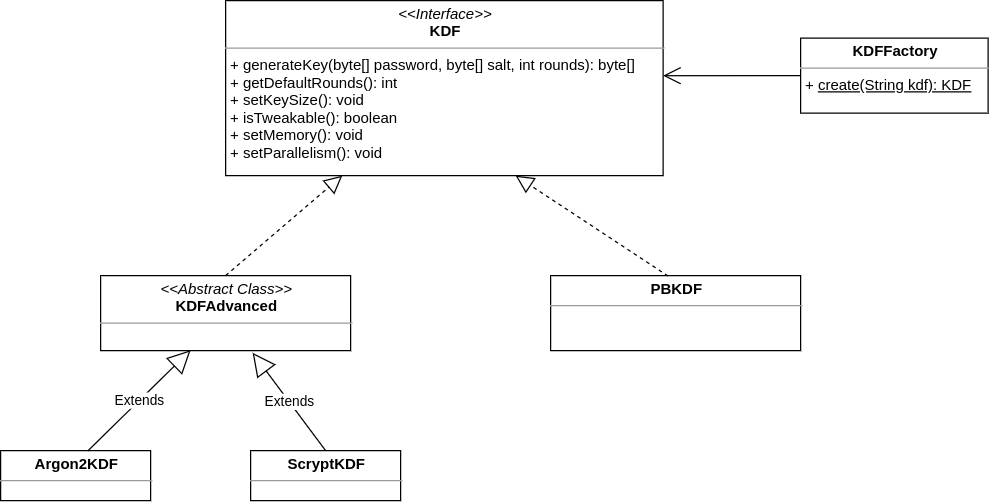
\includegraphics[width=\textwidth]{kdf}
\caption{rappresentazione UML del pattern factory per creare un KDF}
\end{figure}

\textbf{Argon2} e \textbf{Scrypt} estendono \textbf{KDFAdvanced} poiché i loro
algoritmi permettono di definire parametri extra come il paralellismo e la memoria usata
dal KDF. \textbf{PBKDF2} è un vecchio metodo per generare una chiave dalla password e
l'unico parametro configurabile è il numero di round che usa internamente, per questo
ho settato il campo \texttt{tweakable} a falso.

Per capire perché il pattern \texttt{Factory} è usato sia per creare \textbf{KDF}
e \textbf{CryptoCipher} bisogna prima analizzare il parsing dell'header e la relativa
encryption/decryption del database.

\subsection*{KDB}

Per progettare questa parte non ho usato le interfacce perché:
\begin{itemize}
  \item Ho solo una implementazione disponibile.
  \item Sono più flessibile quando devo cambiare la signature di un metodo, senza dover usare un IDE o un LSP per il refactoring.
  \item Principio \href{https://en.wikipedia.org/wiki/You_aren%27t_gonna_need_it}{YAGNI} e \href{https://en.wikipedia.org/wiki/KISS_principle}{KISS}.
\end{itemize}

\textbf{KDBHeader} è la classe che si occupa di:
\begin{itemize}
  \item Parsare l'header (Lettura).
  \item Configurare i vari parametri (Scrittura).
\end{itemize}

\textbf{KDB} è la classe che tramite il \textbf{KDBHeader} si occupa di cifrare/decifrare
dati arbitrari.
Il pattern factory per \textbf{CryptoCipher} e \textbf{KDF} è utile quando in \textbf{KDB}
si effettua l'operazione \texttt{encrypt} e \texttt{decrypt}. I metodi richiedono
a \textbf{KDBHeader} il valore (String) del \texttt{Cipher} e del \texttt{KDF} che viene
passato come parametro di \{Cipher,KDF\}Factory.create() per generare l'oggetto
richiesto.
I due metodi pubblici principali di \textbf{KDB} sono:
\begin{itemize}
  \item \texttt{write}: che esegue l'encryption dell'array di byte in input e lo scrive sul file.
  \item \texttt{read}: che legge il file e lo decrypta. Questo metodo lancia un
    \texttt{IOException} se il file non esiste o un \texttt{AEADBadTagException} quando il file è corrotto.
    Il file può risultare corrotto o perché la password è sbagliata o perché è stato effettivamente manipolato.
    Non lancio tipi diversi di eccezioni (es. \texttt{BadPaddingException}) in base a vari tipi di errore,
    per evitare vari tipi di attacchi (praticamente difficili, ma teoricamente possibili) come
    il padding oracle.
\end{itemize}

\begin{figure}[h]
\centering{}
\includegraphics[width=\textwidth]{kdb}
\caption{rappresentazione UML di KDB}
\end{figure}

\chapter{Sviluppo}
\section{Testing automatizzato}

Durante lo sviluppo del nostro progetto abbiamo utilizzato \texttt{Junit} per
testare il corretto funzionamento delle varie classi.
\textbf{Funzionalità testate automaticamente}:
\begin{itemize}
  \item \textit{CryptoCipher}: viene testato il corretto comportamento dei vari cipher utilizzando lo specifico \texttt{Factory}.
  \item \textit{KDF}: vengono testate le varie KDF utilizzando lo specifico \texttt{Factory}.
  \item \textit{Crypto Util}: test di varie utility per crittografia, come il PKCS\#7 padding e SHA256.
  \item \textit{KDBHeader}: viene testato il corretto funzionamento del \textbf{KDBHeader}, settando vari parametri e controllando il corretto funzionamento dei getter.
  \item \textit{KDB}: test sulla scrittura e lettura di diverse combinazioni di \texttt{cipher} e \texttt{KDF}.
\end{itemize}

I test vengono eseguiti anche in remoto tramite l'apposita \textit{bitbucket pipelines} che
esegue la build del progetto e lancia i vari test.

\section{Metodologia di lavoro}

TODO.

\section{Note di sviluppo}

\section*{Giovanni Di Santi}

\begin{itemize}
  \item \textit{javax.crypto e java.security}: usata per lavorare con Cipher, KDF, e MessageDigest.
  \item \textit{Stream}: usata per manipolare l'header in modo efficace ed elegante.
  \item \textit{Libreria Google Guava}: lavorare con i byte array in java non è comodo. Questa libreria ha varie classi per semplificare
    il lavoro tra cui \href{https://guava.dev/releases/19.0/api/docs/com/google/common/primitives/Bytes.html}{Bytes}.
  \item \textit{ByteBuffer}: per convertire in little endian i bytes, i Data\{Input,Output\}Stream in java lavorano solo in big-endian.
  \item \textit{Libreria Argon2 e Scrypt}: Questi due KDF non erano disponibili dentro \texttt{javax.crypto}.
  \item \textit{Libreria Apache Commons}: per convertire byte array in formato esadecimale.
\end{itemize}

\chapter{Commenti finali}

In quest'ultimo capitolo si tirano le somme del lavoro svolto e si delineano eventuali sviluppi 
futuri.

\textit{Nessuna delle informazioni incluse in questo capitolo verrà utilizzata per formulare la valutazione finale}, a meno che non sia assente o manchino delle sezioni obbligatorie.
%
Al fine di evitare pregiudizi involontari, l'intero capitolo verrà letto dai docenti solo dopo aver formulato la valutazione.

\section{Autovalutazione e lavori futuri}

\subsection*{Giovanni Di Santi}

L'idea iniziale del progetto è stata mia perché mi piace lavorare con la crittografia.
Mi è piaciuto come ho realizzato la parte di \textbf{CryptoCipher}, tuttavia l'architettura
che riguarda \textbf{KDF} non mi risulta ottimale. Un difetto che ho trovato
è stata l'integrazione manuale dei vari metodi in \textbf{KDF} dentro gli accessor
method di \textbf{KDBHeader}.  Dovrebbero esistere librerie, plugin o pattern di
programmazione su misura per quel tipo di problema ma non li ho usati.
In \textbf{KDB} non ho aderito al Single-responsibility principle (SRP) per comodità,
infatti la classe effettua sia la \texttt{write} che la \texttt{read}, al posto di suddividere
i compiti in due classi diverse. L'ho fatto principalmente perché entrambi i metodi
usano lo stato dell'oggetto (campi) per essere eseguiti, quindi era molto conveniente tenerli all'interno
della stessa classe.
Ho dovuto lavorare di più del dovuto perché i miei compagni fino a settembre
non hanno implementato nessuna parte di codice significativo.
A inizio giugno la modellazione e l'implementazione della maggior parte del mio
compito erano completate, tuttavia mi sono ritrovato ad aggiungere parti di 
codice in più a settembre, poiché i miei compagni hanno iniziato a lavorare
solo in quel mese. Vari problemi sarebbero nati subito se avessimo lavorato
insieme. Ad esempio ho dovuto aggiungere vari metodi che aiutassero Francesco a modellare
la GUI, difatti tutti i miei commit di settembre sono getter e setter aggiuntivi.
Avendo progettato l'architettura abbastanza bene non ho avuto problemi ad aggiungere
quelle parti di codice, tuttavia ho dovuto riprendere in mano un codice scritto 3 mesi
prima e continuare a lavorarci sopra. Avrei preferito consegnare con la deadline C.

\appendix
\chapter{Guida utente}

Capitolo in cui si spiega come utilizzare il software. Nel caso in cui il suo uso sia del tutto 
banale, tale capitolo può essere omesso.
%
A tal riguardo, si fa presente agli studenti che i docenti non hanno mai utilizzato il software 
prima, per cui aspetti che sembrano del tutto banali a chi ha sviluppato l'applicazione possono non 
esserlo per chi la usa per la prima volta.
%
Se, ad esempio, per cominciare una partita con un videogioco è necessario premere la barra 
spaziatrice, o il tasto ``P'', è necessario che gli studenti lo segnalino.

\subsection*{Elementi positivi}

\begin{itemize}
 \item Si istruisce in modo semplice l'utente sull'uso dell'applicazione, eventualmente facendo uso di schermate e descrizioni.
\end{itemize}

\subsection*{Elementi negativi}
\begin{itemize}
 \item Si descrivono in modo eccessivamente minuzioso tutte le caratteristiche, anche minori, del software in oggetto.
 \item Manca una descrizione che consenta ad un utente qualunque di utilizzare almeno le funzionalità primarie dell'applicativo.
\end{itemize}

\bibliographystyle{abbrv}
\bibliography{template}

\end{document}

